% Options for packages loaded elsewhere
\PassOptionsToPackage{unicode}{hyperref}
\PassOptionsToPackage{hyphens}{url}
\documentclass[
  american,
  12pt,
  letterpaper,
]{article}
\usepackage{xcolor}
\usepackage{amsmath,amssymb}
\setcounter{secnumdepth}{5}
\usepackage{iftex}
\ifPDFTeX
  \usepackage[T1]{fontenc}
  \usepackage[utf8]{inputenc}
  \usepackage{textcomp} % provide euro and other symbols
\else % if luatex or xetex
  \usepackage{unicode-math} % this also loads fontspec
  \defaultfontfeatures{Scale=MatchLowercase}
  \defaultfontfeatures[\rmfamily]{Ligatures=TeX,Scale=1}
\fi
\usepackage{lmodern}
\ifPDFTeX\else
  % xetex/luatex font selection
\fi
% Use upquote if available, for straight quotes in verbatim environments
\IfFileExists{upquote.sty}{\usepackage{upquote}}{}
\IfFileExists{microtype.sty}{% use microtype if available
  \usepackage[]{microtype}
  \UseMicrotypeSet[protrusion]{basicmath} % disable protrusion for tt fonts
}{}
\makeatletter
\@ifundefined{KOMAClassName}{% if non-KOMA class
  \IfFileExists{parskip.sty}{%
    \usepackage{parskip}
  }{% else
    \setlength{\parindent}{0pt}
    \setlength{\parskip}{6pt plus 2pt minus 1pt}}
}{% if KOMA class
  \KOMAoptions{parskip=half}}
\makeatother
\usepackage{graphicx}
\makeatletter
\newsavebox\pandoc@box
\newcommand*\pandocbounded[1]{% scales image to fit in text height/width
  \sbox\pandoc@box{#1}%
  \Gscale@div\@tempa{\textheight}{\dimexpr\ht\pandoc@box+\dp\pandoc@box\relax}%
  \Gscale@div\@tempb{\linewidth}{\wd\pandoc@box}%
  \ifdim\@tempb\p@<\@tempa\p@\let\@tempa\@tempb\fi% select the smaller of both
  \ifdim\@tempa\p@<\p@\scalebox{\@tempa}{\usebox\pandoc@box}%
  \else\usebox{\pandoc@box}%
  \fi%
}
% Set default figure placement to htbp
\def\fps@figure{htbp}
\makeatother
\ifLuaTeX
\usepackage[bidi=basic,shorthands=off]{babel}
\else
\usepackage[bidi=default,shorthands=off]{babel}
\fi
\ifLuaTeX
  \usepackage{selnolig} % disable illegal ligatures
\fi
\setlength{\emergencystretch}{3em} % prevent overfull lines
\providecommand{\tightlist}{%
  \setlength{\itemsep}{0pt}\setlength{\parskip}{0pt}}
\usepackage[margin=1.24in]{geometry}
\usepackage{setspace}
\usepackage{graphicx}
\usepackage{xcolor}
\usepackage{helvet}
\usepackage{titlesec}
\usepackage{fancyhdr}
\usepackage{booktabs}
\usepackage{longtable}
\usepackage{array}
\usepackage{hyperref}
\definecolor{BookGold}{HTML}{FFD166}
\definecolor{BookBone}{HTML}{F6E8C8}
\definecolor{BookEmber}{HTML}{FF5E3A}
\definecolor{BookInk}{HTML}{12171F}
\renewcommand{\familydefault}{\rmdefault}
\setstretch{1.31}
\setlength{\parindent}{0pt}
\setlength{\parskip}{1.05em}
\raggedbottom
\titleformat{\section}{\normalfont\Large\bfseries\sffamily\color{BookEmber}}{\thesection}{0.7em}{}
\titleformat{\subsection}{\normalfont\large\bfseries\sffamily\color{BookGold}}{\thesubsection}{0.7em}{}
\hypersetup{
  colorlinks=true,
  linkcolor=BookEmber,
  urlcolor=BookEmber,
  citecolor=BookEmber
}
\pagestyle{fancy}
\fancyhf{}
\fancyhead[L]{\sffamily\small\textcolor{BookInk}{Children of the Feed}}
\fancyhead[R]{\sffamily\small\textcolor{BookInk}{\nouppercase{\leftmark}}}
\fancyfoot[C]{\sffamily\small\thepage}
\setlength{\headheight}{14pt}
\usepackage{bookmark}
\IfFileExists{xurl.sty}{\usepackage{xurl}}{} % add URL line breaks if available
\urlstyle{same}
% fallback for those not using the hyperref driver hyperxmp:
\makeatletter
\@ifundefined{xmpquote}{\newcommand{\xmpquote}[1]{#1}}{}
\makeatother
\hypersetup{
  pdftitle={We Were the Dataset},
  pdflang={en-US},
  hidelinks,
  pdfcreator={LaTeX via pandoc}}

\title{We Were the Dataset}
\author{}
\date{}

\begin{document}
\maketitle

\section{We Were the Dataset}\label{we-were-the-dataset}

\subsection{Deck}\label{deck}

First they captured what we made. Then they captured how we think.

\begin{figure}
\centering
\pandocbounded{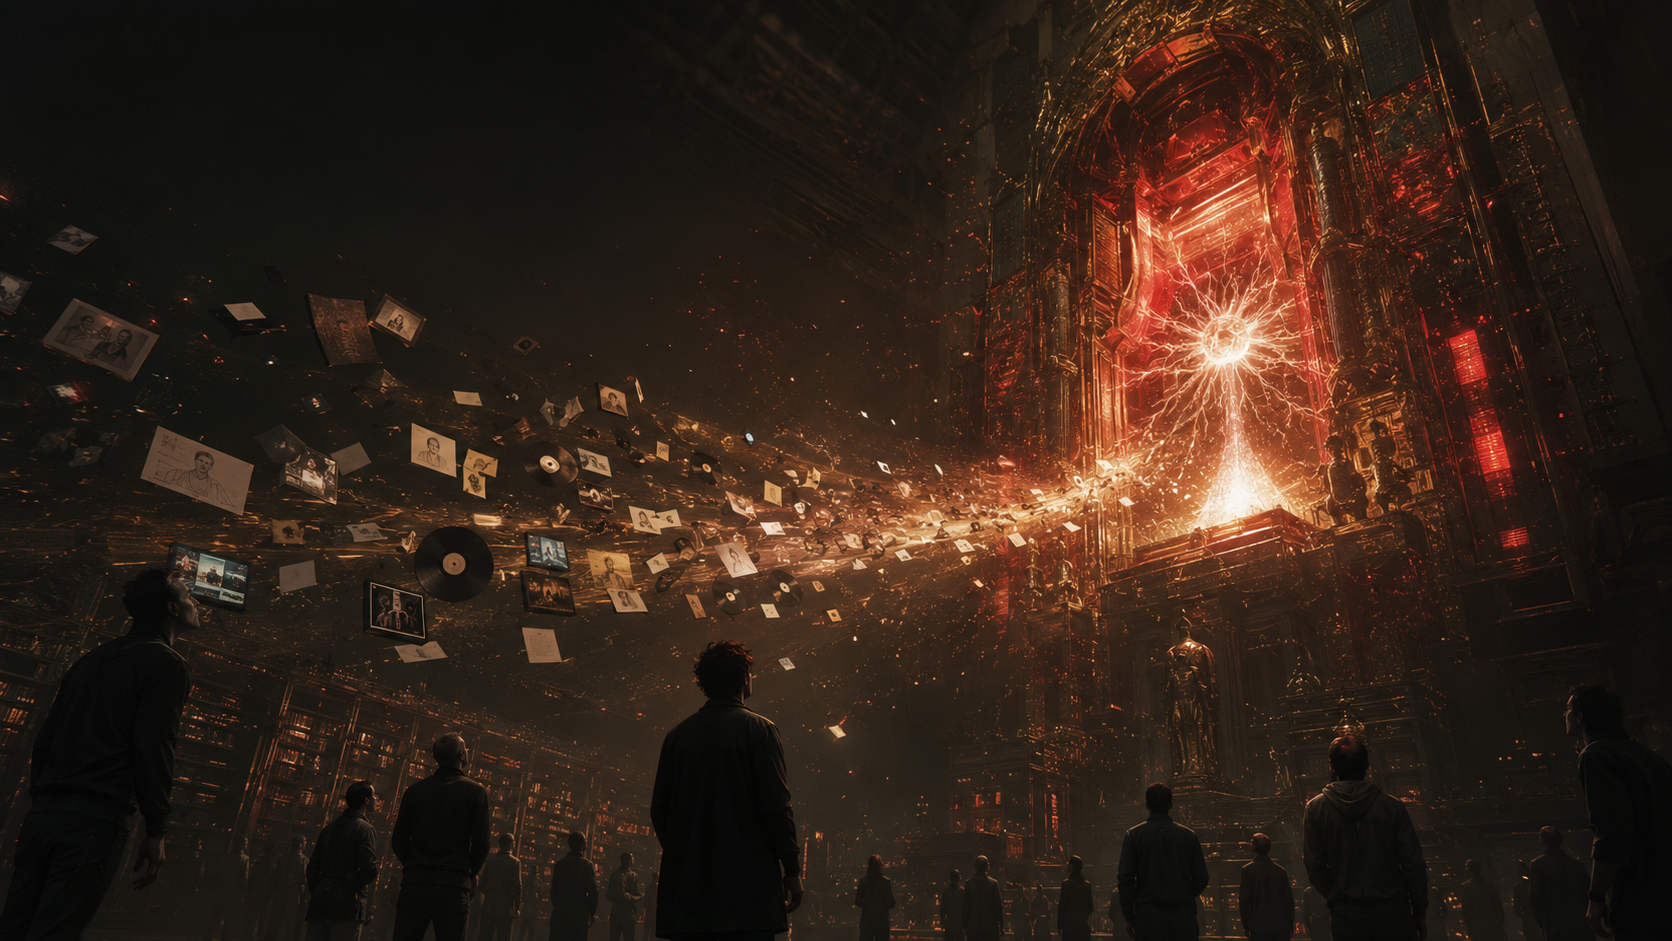
\includegraphics[keepaspectratio,alt={Chapter 04 cover}]{../assets/generated/covers/04_we-were-the-dataset_cover.png}}
\caption{Chapter 04 cover}
\end{figure}

\subsection{Opening}\label{opening}

They did not build the AI god from nothing.

They built it from our searches, our books, our fan edits, our code
commits, our forum fights, our memes, our DMs, our grief posts, our
playlists, our horny late-night questions, our bug fixes, our lesson
plans, our essays, our jokes, our documentation, our voice notes, our
mistakes, and the endless trail of language we left behind because
digital life had already become compulsory.

That sentence is doing a lot of work, so let's slow it down.

The claim is not that every output from a model is a haunted copy of one
person's work.

The claim is not that weights are literal scrapbooks with names
attached.

The claim is not that math itself is evil.

The claim is that frontier capability is downstream of mass human
contribution, and the political meaning of that contribution was buried
under the language of neutral computation for as long as possible.

\subsection{Main Narrative}\label{main-narrative}

This is the hinge chapter because it explains why social media, platform
extraction, and AI cannot be treated as separate stories anymore. The
earlier platform era created the conditions under which expression
became massively collectible. The model era created the conditions under
which that archive could be condensed into strategic capability.

That movement from archive to capability is the real scandal.

We tend to talk about data as if it were a warehouse category. Data
sounds dry. Administrative. Kind of boring. But most of what mattered in
the training explosion was not boring at all. It was human culture in
active form. Speech, style, humor, expertise, taste, pedagogy, argument,
intimacy, and craft. The machine got fluent because people were already
pouring themselves into systems that could store the evidence of fluency
at scale.

The quiet trick was that unpaid contribution had already been normalized
long before most people cared about model training. Open a platform.
Improve the answer thread. Fix the typo. Add the wiki note. Post the
tutorial. Upload the review. Tag the image. Label the clip. React to the
product. Answer the stranger. Build the open-source library. Debate the
edge case. Explain the concept for free because someone somewhere might
benefit. All of that felt like culture, community, or just ordinary
internet life.

And it was.

But it was also substrate.

\begin{figure}
\centering
\pandocbounded{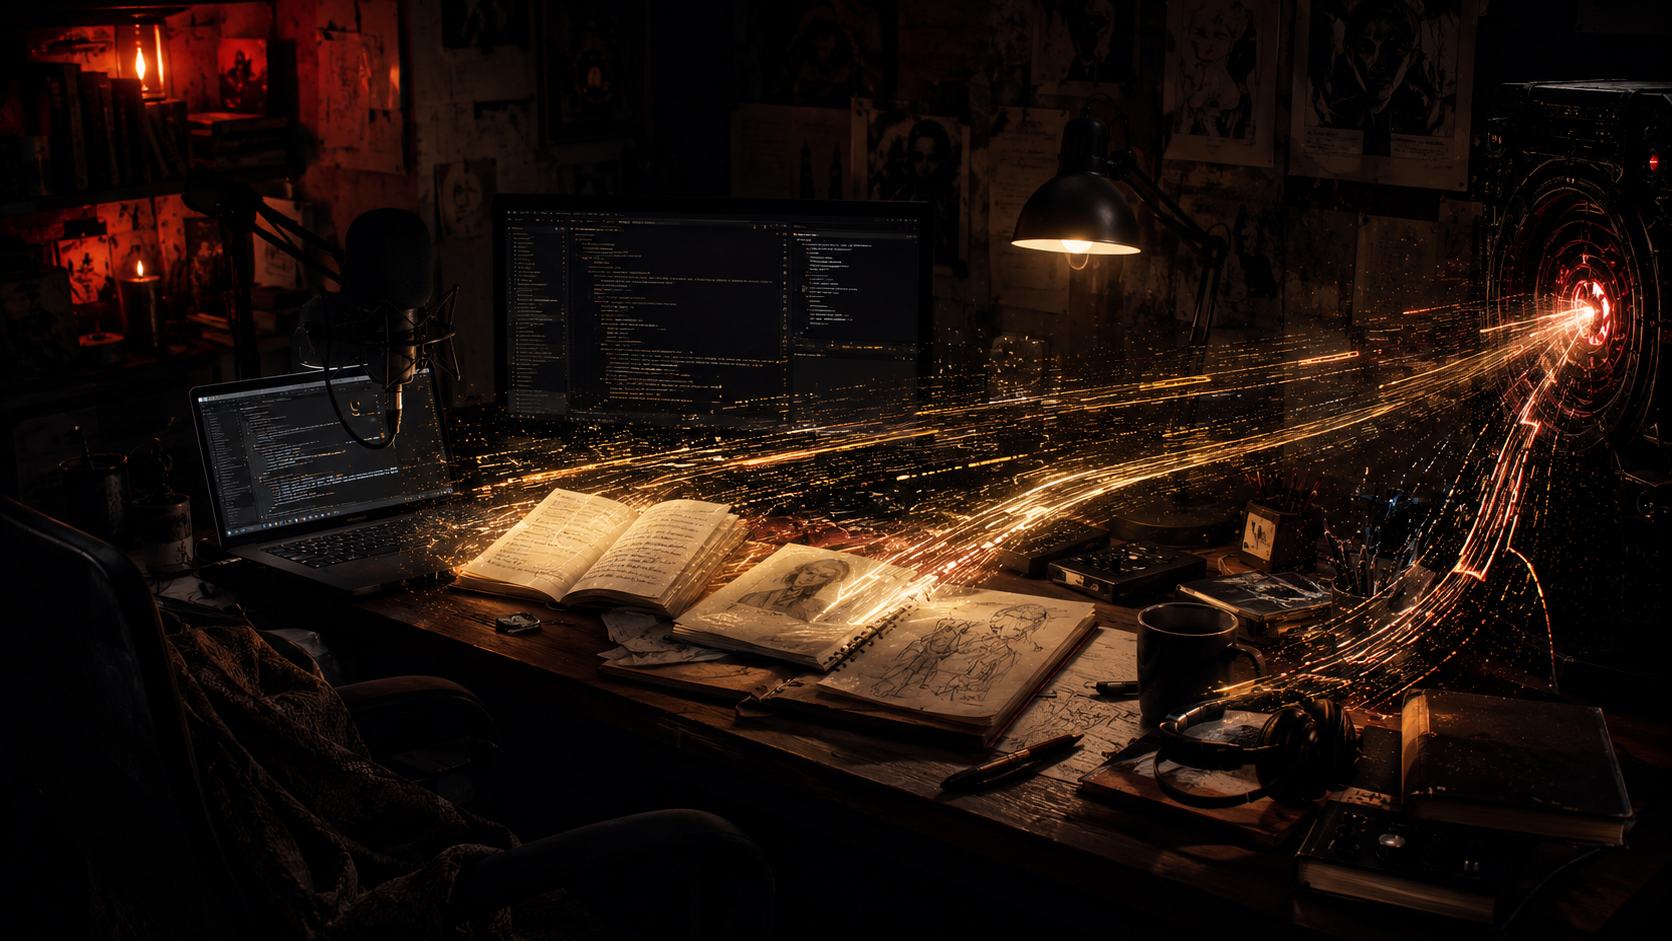
\includegraphics[keepaspectratio,alt={Chapter 04 narrative illustration A}]{../assets/generated/illustrations/04_we-were-the-dataset_scene_a.png}}
\caption{Chapter 04 narrative illustration A}
\end{figure}

That is what changes once the model arrives. The same web that looked
messy and alive from the human side starts looking like ingestible
pattern from the machine side. Search becomes corpus. Conversation
becomes training material. Creativity becomes signal. The messy
abundance of public life becomes a commercially valuable precondition.

The industry likes to hide behind scale because scale makes
responsibility blur. If something was trained on ``the internet,'' the
phrase is vague enough to numb the moral imagination. But the internet
is not a weather pattern. It is people. It is the sediment of people.
Their work, their residue, their language, their unfinished
explanations, their vulnerable performances, their expertise donated to
strangers, their bad takes, their brilliance, their cringe, their labor,
their obsession, their boredom, their care.

If a model becomes useful because enough people left enough of
themselves behind in machine-readable form, then usefulness itself has a
social debt baked into it.

That is where the legal and moral fight around weights becomes
unavoidable.

The industry's preferred framing used to sound something like this:
models learn in a transformative way, they do not store the source like
a zip file, and the output is not a one-to-one replay, so calm down.

That argument is not nothing. Some of it speaks to real technical
distinctions. But it is also wildly incomplete as a moral theory.
Because even if a weight is not a memory in the human sense, it is still
a trace of exposure. It is still what remains when a machine has
statistically internalized enough human material to produce synthetic
competence. The exact legal status is contested. The social reality is
not.

A frontier model does not emerge above civilization.

It emerges through civilization.

And that means the emotional experience of AI is not just wonder. It is
estrangement. A lot of people meet these systems and feel two things at
the same time: fascination at the fluency and a low, ugly recognition
that something intimate was abstracted out of ordinary life and turned
into strategic property. That is why so many creators, teachers, coders,
and hyper-online workers feel not only threatened but weirdly gaslit.
They are told the machine is just progress, while quietly recognizing
fragments of the public world that made the progress possible.

That matters for creators first, but not only creators. Writers,
artists, coders, musicians, teachers, forum contributors, researchers,
volunteer moderators, documentation nerds, and just extremely online
people all helped create the world the model could learn from. Some were
paid by institutions. Many were not. A shocking amount of the internet's
most useful material was created by people who believed they were
contributing to public culture, open knowledge, fandom, community, or
personal visibility, not furnishing private power for the next
intelligence hierarchy.

That is why the term patrimony becomes so important in the broader
argument. Not because it sounds fancy. Because it names a category
between ``nobody owns this'' and ``a small number of firms get to own
this completely.'' If frontier capability is built from humanity's
collective archive, then treating the result as ordinary private
property by default starts to look less like innovation and more like
enclosure.

\begin{figure}
\centering
\pandocbounded{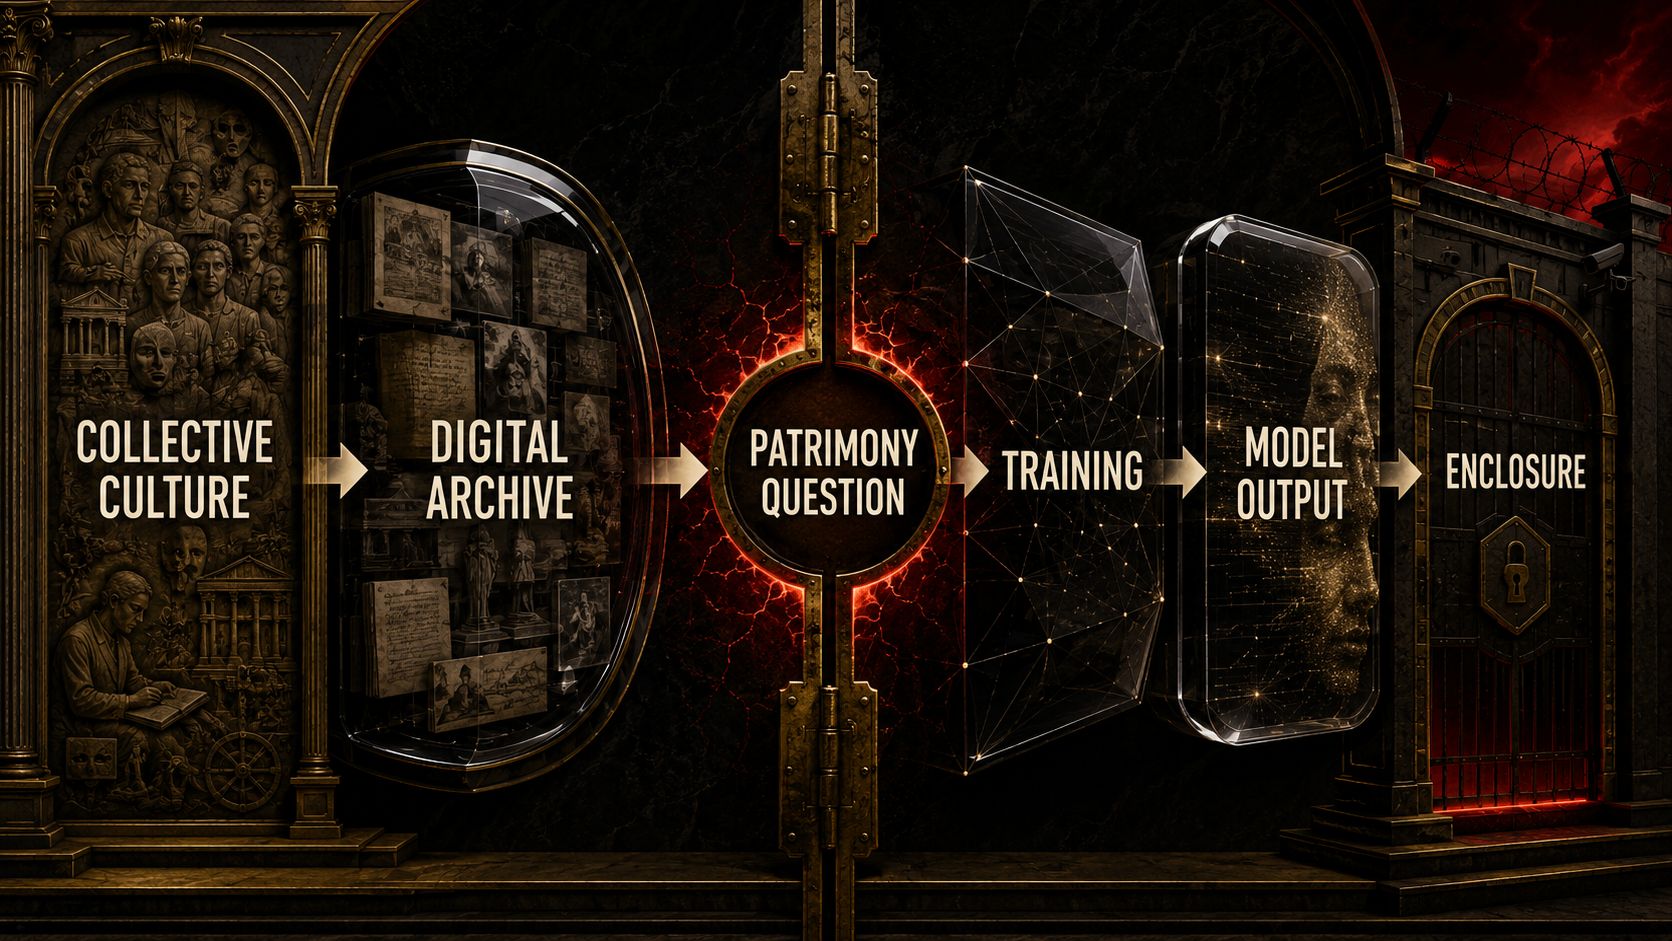
\includegraphics[keepaspectratio,alt={Chapter 04 archive enclosure infographic}]{../assets/generated/infographics/04_we-were-the-dataset_infographic_b.png}}
\caption{Chapter 04 archive enclosure infographic}
\end{figure}

\begin{figure}
\centering
\pandocbounded{
\includegraphics[keepaspectratio,alt={Chapter 04 infographic}]{../assets/generated/infographics/04_we-were-the-dataset_infographic_a.png}}
\caption{Chapter 04 infographic}
\end{figure}

The politics of licensing complicate the story even further. Once the
value of the archive becomes undeniable, firms start trying to
regularize what was previously extracted under looser assumptions. This
is where the Reddit example matters. A large social platform is no
longer just a forum in this story. It becomes proof that collective
human conversation can be enclosed twice: first as unpaid behavioral or
cultural residue, then again as a licensable asset for model
development.

That double enclosure is one of the ugliest moves in the whole cycle.

First the system convinces people to generate the field.

Then it convinces the world the field is a commodity.

Then it sells the field back as capability.

Then it tells the people who generated it that the resulting machine is
progress and maybe also their replacement.

That is not a clean innovation story.

That is empire logic with better branding.

And it is not only an ownership story. It is also a shelf story.

Supermarkets did not need to invent the tomato. They needed to control
the shelf where the tomato was sold. AI firms are learning a similar
move with cognition. They do not need to outlive every artist, every
programmer, every writer, or every expert in a pure merit contest. They
need to become the first interface the customer reaches. The prompt box,
the chatbot, the subscription layer, the clean white rectangle on the
screen: that is the new shelf.

Once the shelf controls first contact, the value fight changes. Human
work does not have to become worthless to become weaker. It only has to
become easier to price downward. The creator is still there. The craft
is still there. The judgment is still there. But the interface now
stands between the creator and the customer, and that is enough to start
renegotiating what the human on the other side is supposedly worth.

It is also why the politics of consent cannot be reduced to some fantasy
of perfect individual opting in. Most people did not meaningfully
negotiate with the systems that absorbed their residue. They lived,
posted, coded, taught, uploaded, commented, revised, joked, and worked
inside environments that had already become necessary for participation.
``Consent'' in that context often means something closer to procedural
surrender. You click through because the social and economic world is
already routed through the stack. Later, that routinized surrender gets
reframed as if the archive simply existed, ownerless and ready for
compression by whoever reached scale first.

\begin{figure}
\centering
\pandocbounded{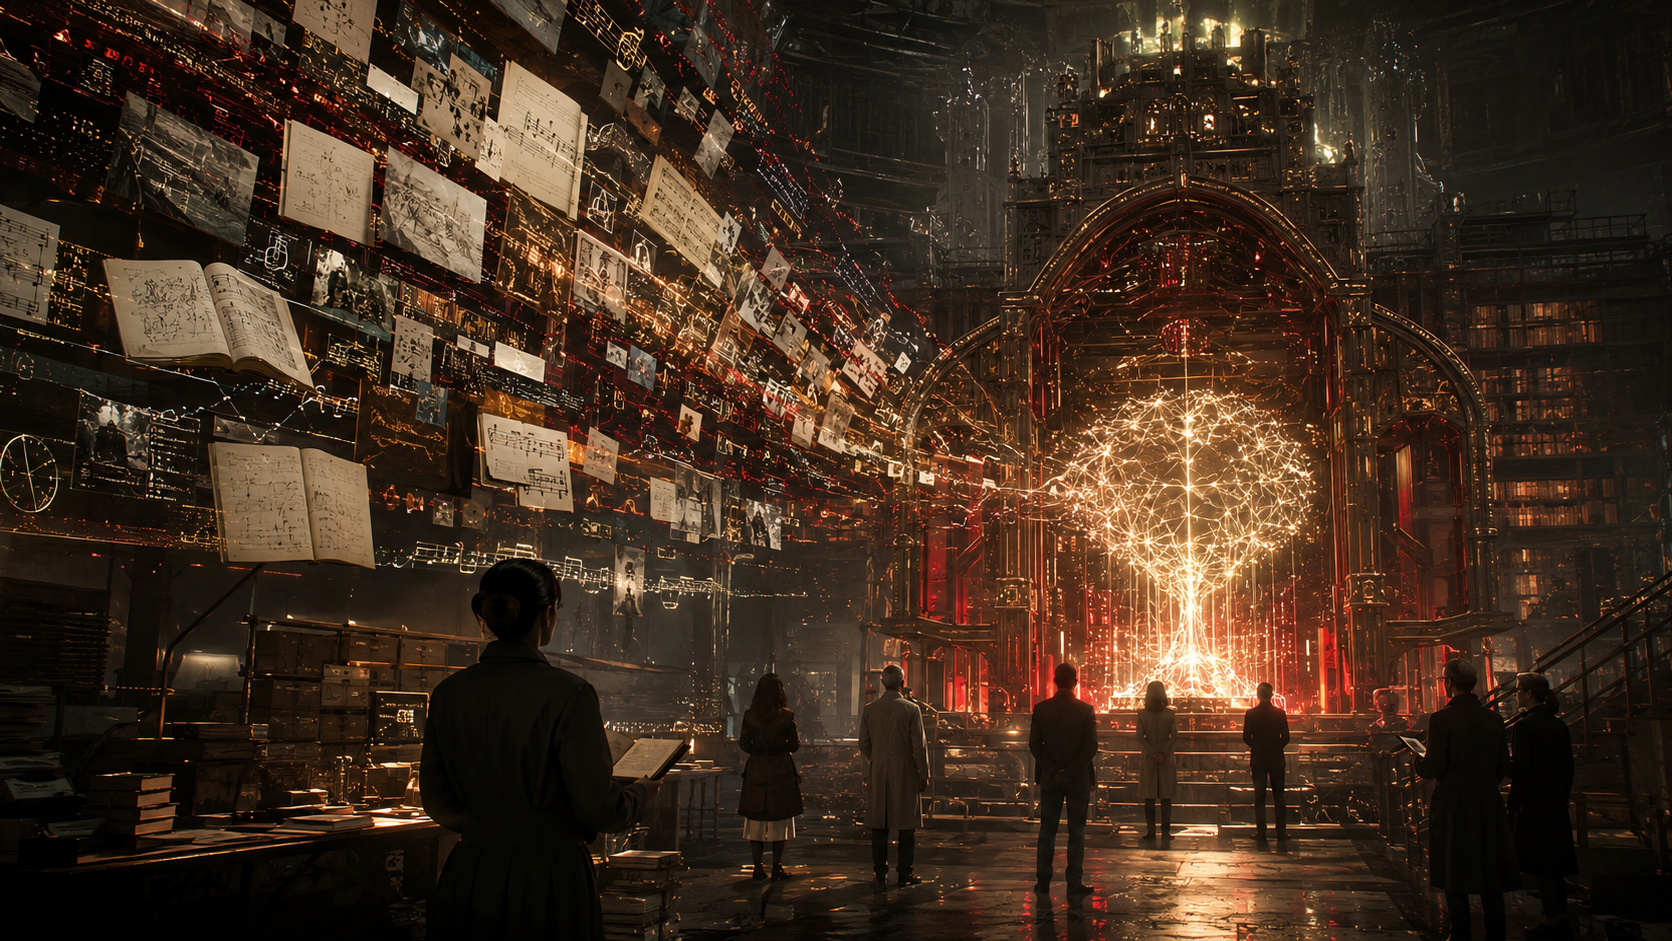
\includegraphics[keepaspectratio,alt={Chapter 04 narrative illustration}]{../assets/generated/illustrations/04_we-were-the-dataset_scene.png}}
\caption{Chapter 04 narrative illustration}
\end{figure}

\begin{figure}
\centering
\pandocbounded{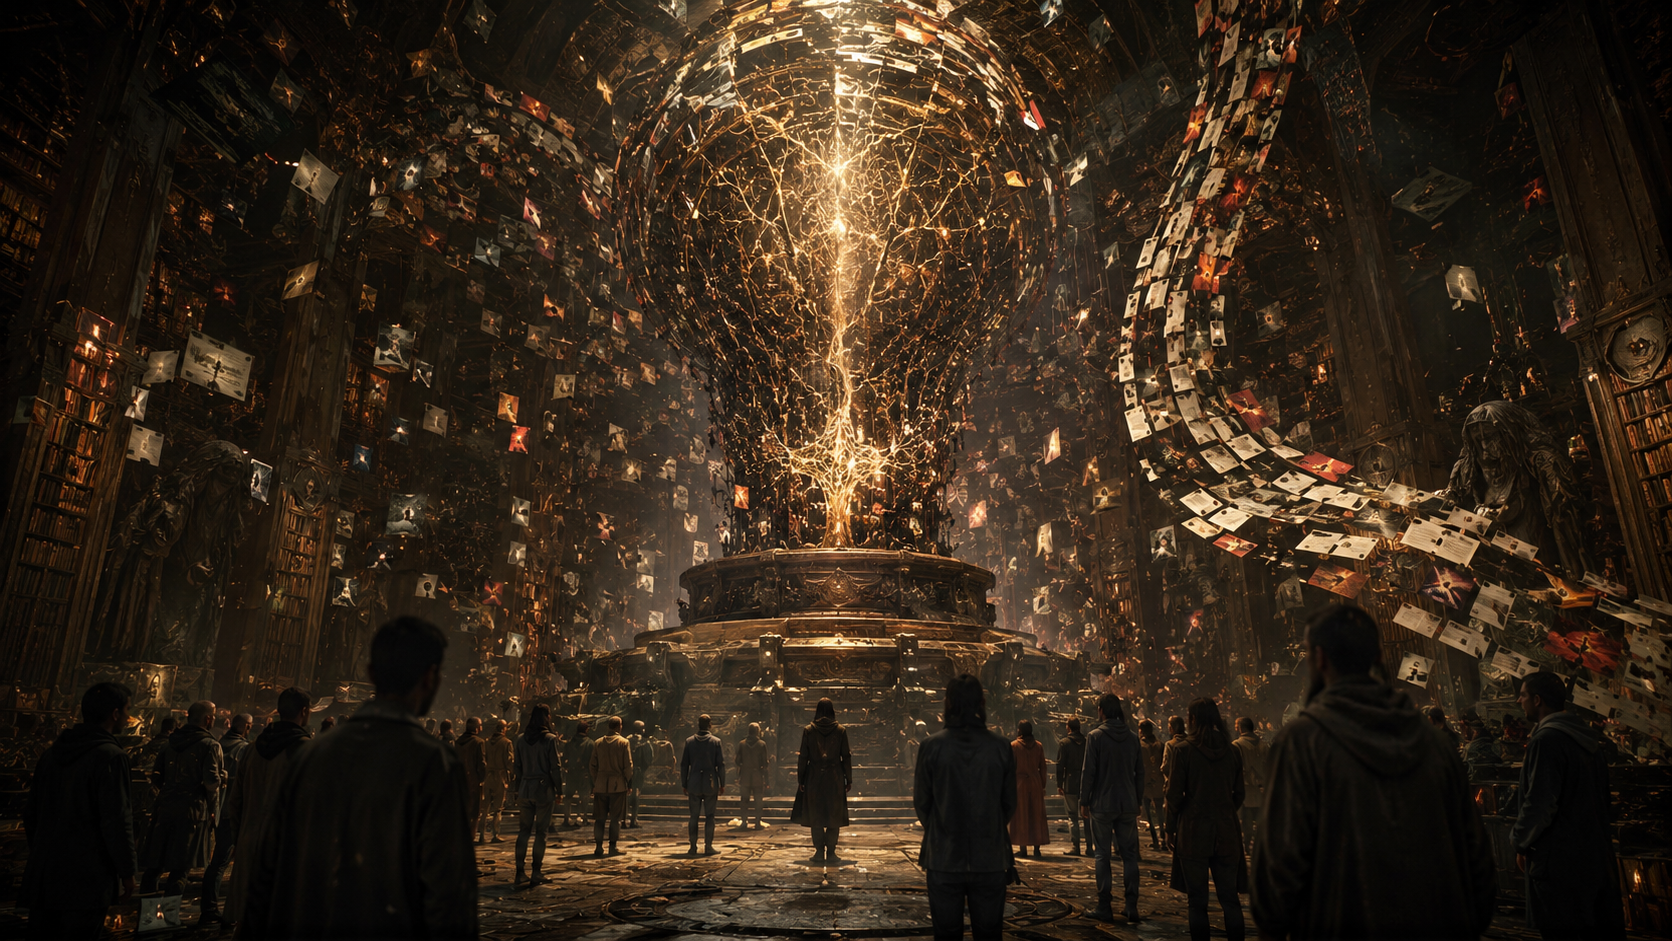
\includegraphics[keepaspectratio,alt={Chapter 04 narrative illustration B}]{../assets/generated/illustrations/04_we-were-the-dataset_scene_b.png}}
\caption{Chapter 04 narrative illustration B}
\end{figure}

This is also the chapter where the emotional tone of the book changes a
little. Up to this point, a reader could still maintain some distance
and think, okay, platforms got creepy, social life got weird, the
pandemic accelerated bad habits, sure. But here the realization gets
personal in a different way. The machine is not only around us. It is
made from what we already gave away, often without understanding the end
use, sometimes without a meaningful alternative, and almost never under
conditions of real bargaining power.

That is why people feel a particular kind of insult when AI products are
introduced as if they arrived through pure genius. Of course there is
real engineering. Of course some technical leaps are genuine. But genius
did not produce the archive. Society did. Users did. Workers did.
Creators did. The culture did. The machine inherits the labor of the
species and then reappears under a corporate logo.

Once you see that, the ownership question becomes impossible to dodge.

If human civilization was the training field, who should govern the
resulting capability?

If the archive was collectively generated, should the output be
permanently enclosed by whoever had enough capital and compute to
compress it first?

If the public supplied the substrate, what obligations attach to the
machine?

These are not abstract future questions anymore. They are already
showing up in fights over copyright, licensing, model access, public
funding, state partnership, and who gets to speak with the authority of
synthetic intelligence.

The interpretation advanced in this project is not that current law has
already settled the matter in favor of public patrimony.

It absolutely has not.

The interpretation is that the law is lagging a moral reality that is
already visible: weights built from collective human expression should
not simply inherit the default moral status of ordinary proprietary
assets.

That is not anti-technology.

It is anti-enclosure.

And unless that distinction becomes politically legible, the next phase
of the AI economy will keep repeating the same move: privatize what was
socially produced, then market access to it as destiny.

\subsection{Research Basis}\label{research-basis}

This chapter adapts the documentary argument developed in the research
paper
\href{../../papers/html/04_data-models-weights_paper.html}{\textbf{Chapter
04: AI Arrives When the Human Raw Material Already Exists}}. The PDF
version is
\href{../../papers/pdf/04_data-models-weights_paper/04_data-models-weights_paper.pdf}{here}.
That paper grounds the weights debate in Copyright Office records,
memorization research, licensing developments, court conflict, and the
social-to-model bridge.

\subsection{Next}\label{next}

Once the archive becomes commercial capability, the next fight is not
only about creators. It is also about workers. The same industry that
learned from human labor started using AI rhetoric to weaken that labor,
reorganize it, and call the whole process inevitable.

\end{document}
